% !TEX root = ../../prj4projektdokumentation.tex
% SKAL STÅ I TOPPEN AF ALLE FILER FOR AT MASTER-filen KOMPILERES 

\section{Blok definitionsdiagram}
Et BDD for spændingsregulator ses på figur \ref{fig:BDDSpaendingsregulator}. På diagrammet ses de overordnede blokke, spændingsregulator består af. En beskrivelse af hver blok kan læses under figur \ref{fig:BDDSpaendingsregulator}.

\begin{figure}[htbp] % (alternativt [H])
	\centering
	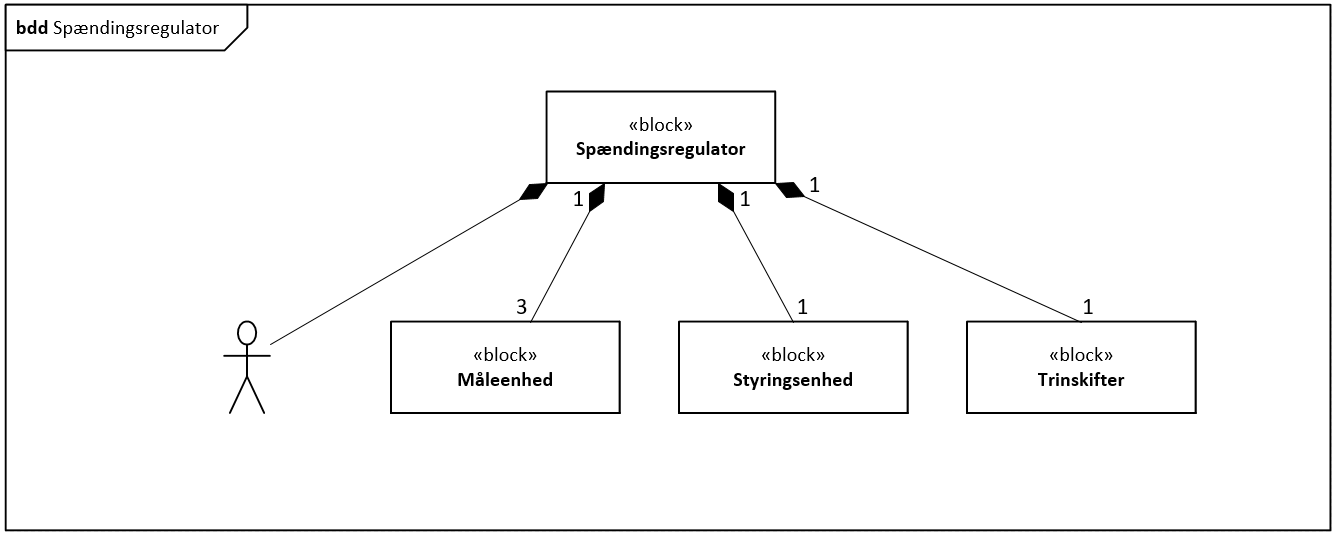
\includegraphics[width=0.9\textwidth]{Figure/BDDSpaendingsregulator}
	\caption{BDD Spændingsregulator}
	\label{fig:BDDSpaendingsregulator}
\end{figure}

\textbf{Måleenhed} står for at måle spænding, strøm og faseforskydningen herimellem. Ligeledes skal denne kunne måle indholdet af harmoniske frekvenser. Den skal bestå af hardware til måling af de nævnte parametre og en PSoC. På enheden skal behandlingen af rådataet også ligge, så dette kan formidles til styringsenheden.

\textbf{Styringsenhed} har til opgave at styre trinskifteren ud fra de data den får fra målenehderne. Den består af en PLC, der skal kommunikerer med brugergrænsefladen, så en bruger kan følge med i data fra Måleenhederne.

\textbf{Brugergrænsefladen} står for at formidle måledata til brugeren gennem en skærm, men det er også her at brugeren skal kunne interagere med systemet i manuel tilstand.

\textbf{Kommunikationsmodul} skaber en kommunikation fra Måleenhedens PSOC til Styringsenhedens PLC.

\textbf{Kontrolmodul} laves på en PLC, til at styrer trinene på trinskifteren.






\textbf{Trinskifter} er en enhed der kan skifte trin på en transformer ud fra et signal fra styringsenheden. Den skal altså bestå af et relæ for hvert trin, der kan kontrolleres af styringsenheden.